\appendix
\section{Supplementary Material}

% \subsection{Effectiveness of attacks on different codecs.}
% In Fig.~\ref{fig:qd-codecs} and \ref{fig:ced-codecs} are the results across different NIC architectures. They confirm that our attack is broadly effective and generalizes well beyond a single codec family. While traditional methods such as I-FGSM and FTDA show limited degradation ---especially against stronger codecs like JPEG AI --- our modular approach consistently produces higher QD-SCORE values. The inclusion of local artifact amplification and normalized gradient updates proves particularly important for more advanced models, enabling substantial quality degradation even where prior attacks fail. These findings highlight the robustness and versatility of the proposed method across both classic hyperprior models and modern transformer- or GAN-based codecs.
% \begin{figure*}[h!]
% \centering
% \includegraphics[width=.9\textwidth]{images/QDM_rose_cropped.pdf}
% \caption{Comparison of QD-SCORE on different NIC models. Lines represent attack efficiency for the proposed method and other methods.}
% \label{fig:qd-codecs}
% %\vspace*{-0.4cm}
% \end{figure*}

% \begin{figure*}[h!]
% \centering
% \includegraphics[width=.9\textwidth]{images/CEDM_rose_cropped.pdf}\\
% \caption{Comparison of CED-SCORE on different NIC models. Lines represent attack efficiency for the proposed method and other methods.}
% \label{fig:ced-codecs}
% %\vspace*{-0.4cm}
% \end{figure*}

\subsection{Attack invisibility-efficiency trade-off.}
Fig.~\ref{fig:high_bitrate_ex} illustrates the trade-off between invisibility and compression efficiency degradation (CED-SCORE). The results show that our proposed method consistently achieves higher CED-SCORE values at comparable levels of invisibility than baseline attacks, indicating a more effective balance between stealth and destructive impact. In particular, the frequency-domain masking variant attains the best compromise: it maintains imperceptible perturbations while still inducing significant efficiency losses in the codecs. This demonstrates that the modular design not only enhances attack strength but also improves its practicality by minimizing visual detectability.
\begin{figure}[!t]
% \begin{wrapfigure}{l}{0.7\textwidth}
\centering
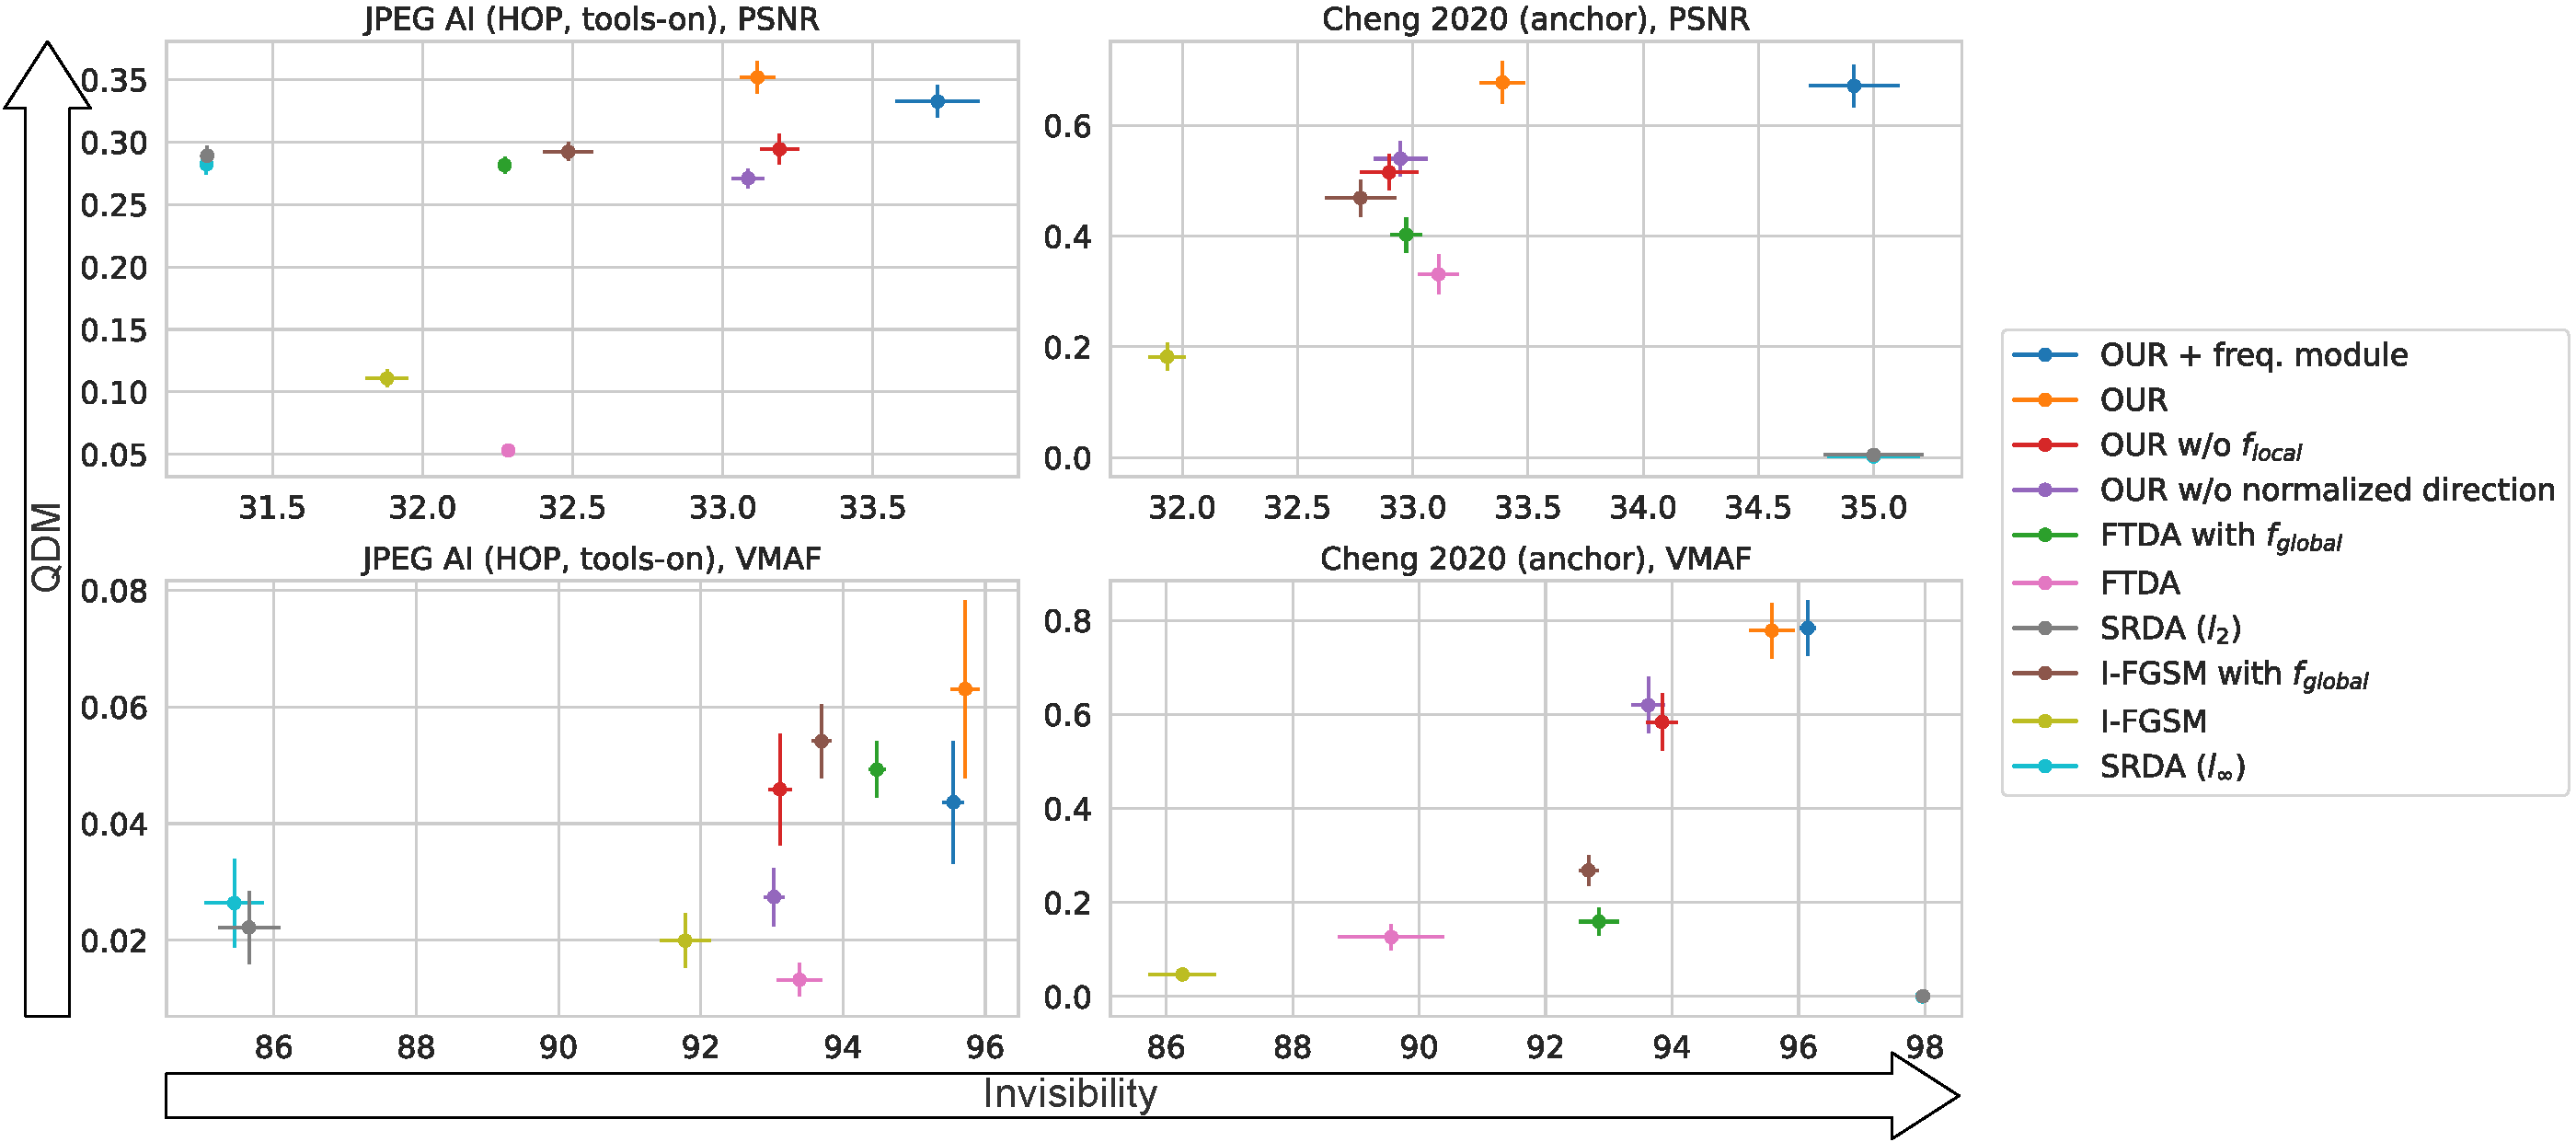
\includegraphics[width=.82\linewidth]{images/Untitled 8_cropped.pdf}
% \subfigure[]{\includegraphics[width=.45\textwidth]{iclr2026/images/Untitled 8_cropped.pdf}}
\caption{Comparison of QDM across different NIC models (with the lowest compression ratio in their families). Our proposed method, particularly with the frequency-domain masking module, consistently achieves higher QDMs while maintaining stealth, outperforming baseline attacks across both classical and modern codecs.}
\label{fig:high_bitrate_ex}
%\vspace*{-0.4cm}
\end{figure}

\subsection{Alternative perturbation budget.}

In this section, we show the results of an experiment on the KODAK PhotoCD dataset with a smaller perturbation budget $\varepsilon =  5/255$ (and $\varepsilon =  0.0003$ for FTDA and SRDA ($l_2$)). The results in the Tables~\ref{table:RES_ALter_1} show that with a lower $\varepsilon$, attacks become much less effective, but our methods still show the best results.

\begin{table}[!t]
\centering
\setlength{\tabcolsep}{3.5pt}
\renewcommand{\arraystretch}{0.88}
\begin{tabular}{l|rr|rr}
\toprule
 & \multicolumn{2}{l|}{$QD\text{-}SCORE$}  & \multicolumn{2}{l}{$CED\text{-}SCORE$} \\
Attack & PSNR & VMAF  & PSNR & VMAF \\
\midrule
OUR + freq. module  & \textbf{0.17} & 0.10 & \textbf{0.21} & 0.11 \\
OUR  & 0.13 & \textbf{0.12} & 0.17 & \textbf{0.14} \\
I-FGSM with $f_{global}$  & 0.10 & 0.10  & 0.11 & 0.12 \\
FTDA with $f_{global}$  & 0.12 & 0.9  & 0.18 & 0.11 \\
I-FGSM & 0.06 & 0.02  & 0.07 & 0.03 \\
FTDA & 0.08 & 0.05  & 0.10 & 0.06 \\
\bottomrule
\end{tabular}
\caption{Comparison of attack performance across all tested NIC codecs on the KODAK PhotoCD dataset with perturbation budget $\varepsilon = 5/255$. QD-SCORE (quality degradation) and CED-SCORE (compression efficiency degradation) are reported for PSNR and VMAF. The proposed method consistently achieves higher degradation with lower visibility than baseline attacks.}
\label{table:RES_ALter_1}
\end{table}


\subsection{Adversarial images example.}
In this section, we present adversarial images before compression that correspond to the examples shown in Fig.~\ref{fig:examples} to assess the visibility of attacks.

\begin{figure}[!t]
\centering
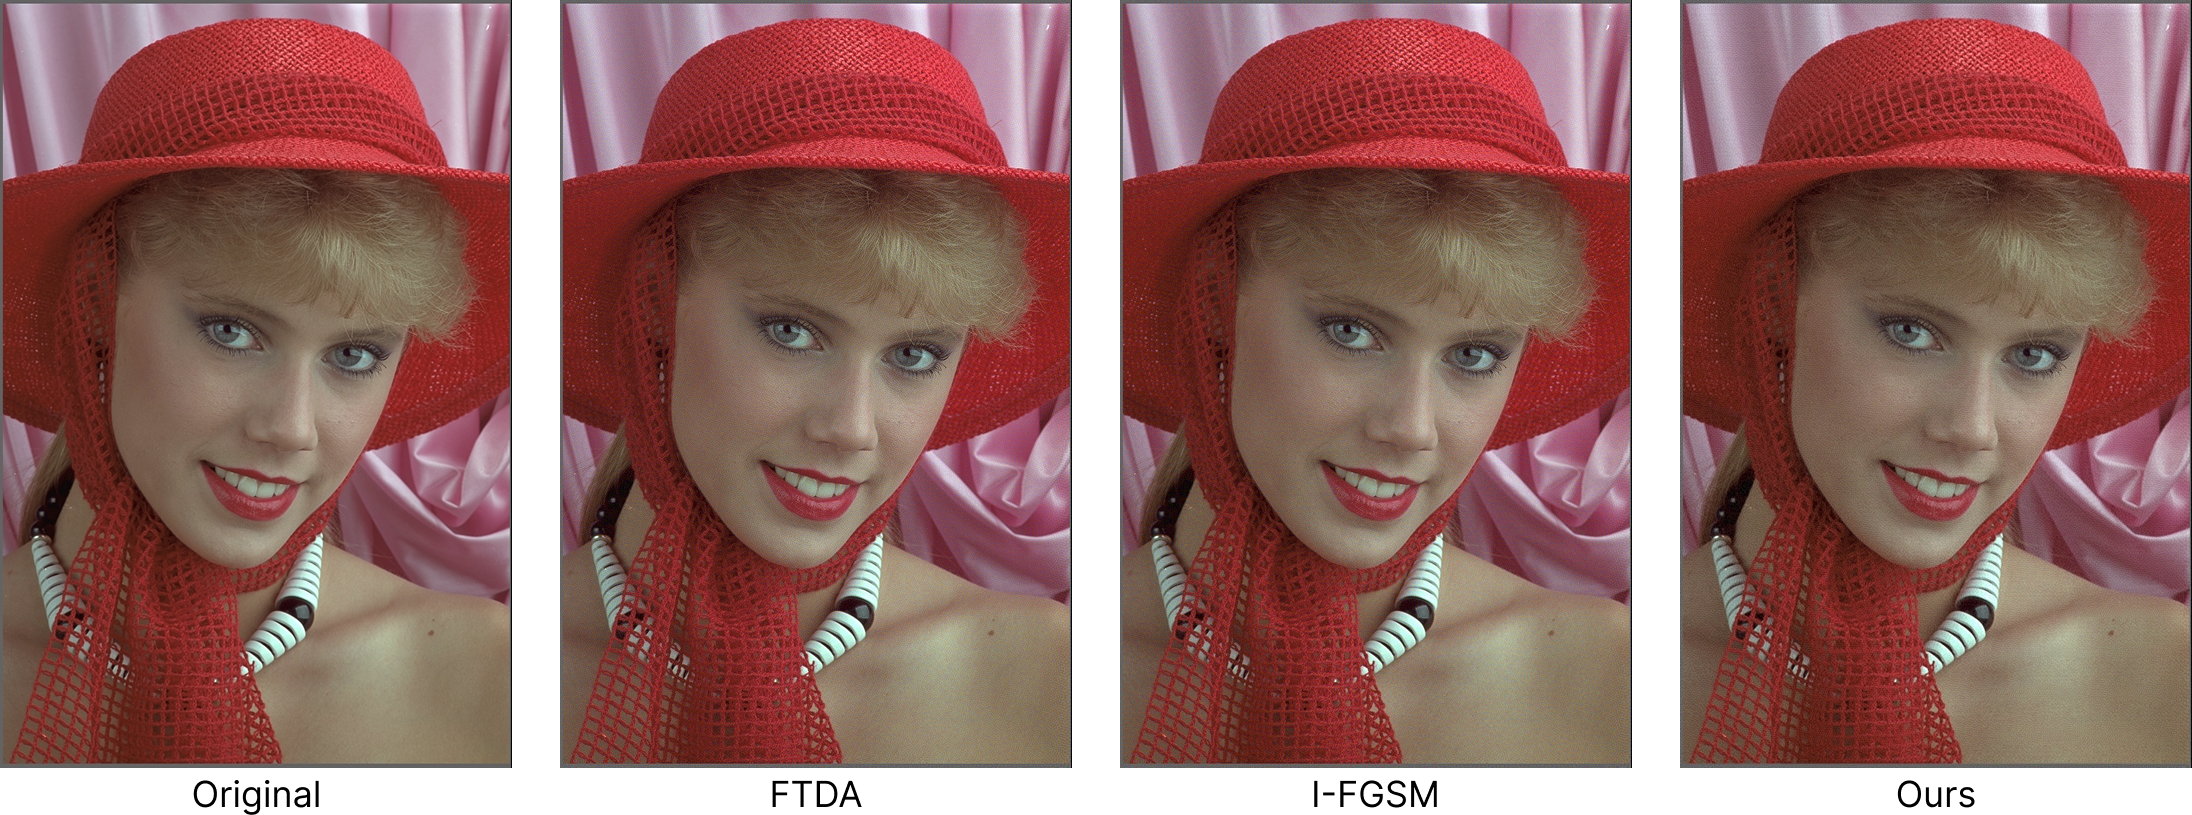
\includegraphics[width=.75\linewidth]{images/example of images with an attack on JPEG AI v7 (HOP).png}
\caption{Adversarial images for JPEG AI v7 (HOP) generated by our proposed attack and compared to baseline methods before compression.}
\label{fig:examples_jpeg}
\end{figure}

\begin{figure}[!t]
\centering
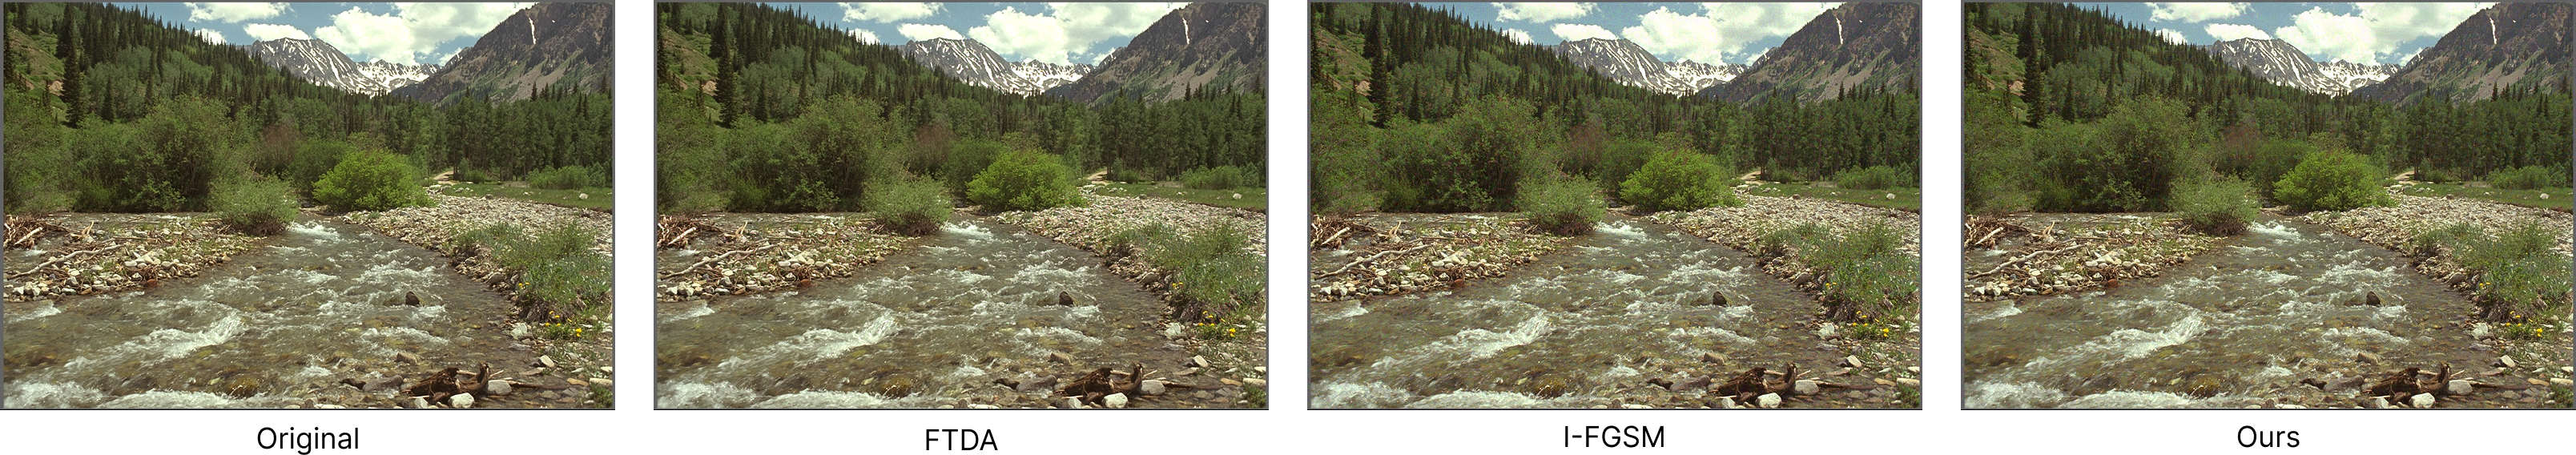
\includegraphics[width=.85\linewidth]{images/example of images with attack on Cheng2020 (attn).png}
\caption{Adversarial images for Cheng2020 (attn) generated by our proposed attack and compared to baseline methods before compression.}
\label{fig:examples_cheng}
\end{figure}

\subsection{Variations of the $P$ parameter.}


\begin{table}[!t]
\centering
\setlength{\tabcolsep}{3.5pt}
\renewcommand{\arraystretch}{0.88}
% \begin{tabular}{l|rr}
% \toprule
%  & \multicolumn{2}{l}{$QD\text{-}SCORE$}  \\
% $P$ & PSNR & VMAF   \\
% \midrule
% 25  & 0.157 & 0.087  \\
% 50  & 0.189 & 0.090 \\
% 75  & 0.188 & 0.090 \\
% 100 & 0.188 & 0.091  \\
% 125 & 0.181 & 0.088  \\
% 150 & 0.177 & 0.089  \\
% \bottomrule
% \end{tabular}
\begin{tabular}{l|rrrrrr}
\toprule
$P$ & 25 & 50 & 75 & 100 & 125 & 150 \\
\midrule
PSNR & 0.157 & 0.189 & 0.188 & 0.188 & 0.181 & 0.177 \\
VMAF & 0.087 & 0.090 & 0.090 & 0.091 & 0.088 & 0.089 \\
\bottomrule
\end{tabular}
\caption{$QD\text{-}SCORE$ of our attack for different $P$ values on the JPEG AI codec family using the KODAK dataset.}
\label{table:RES_P}
\end{table}
% \vspace{-1.1em}

The parameter P controls the trade-off between artifact localization granularity and computational efficiency. Empirical findings during development showed that $P \in \left[50, 100 \right]$ approximately the same results are obtained. It makes no sense to increase the parameter, since the current size is sufficient for local artifacts to occur, and increasing it will only lead to the loss of some of them. We selected $P = 75$ as the midpoint providing optimal balance.


\subsection{Coverage Interpretation of the Local Objective}

We now show that the local objective in Eq.~(10) has a direct
artifact-coverage interpretation. Let the image be divided into
$B$ non-overlapping blocks and assume $0\le m_b\le U$. Define
\begin{align*}
m_b &= \max_{(u,v)\in b}\Delta(u,v), \qquad b=1,\ldots,B, \\
f_{\mathrm{local}} &= \sum_{b=1}^{B}m_b, \\
C(\tau) &= \frac{1}{B}\sum_{b=1}^{B}\mathbf{1}[m_b\ge \tau],
\qquad \tau\in[0,U].
\end{align*}
Here, $m_b$ is the maximum local degradation score in block $b$,
and $C(\tau)$ measures how many spatial blocks contain an artifact
whose strength is at least $\tau$. Since the indicator is equal to
one exactly on the interval $[0,m_b]$, for any $m_b\in[0,U]$ we have
\begin{align*}
m_b &= \int_{0}^{U}\mathbf{1}[m_b\ge\tau]\,d\tau, \\
f_{\mathrm{local}}
&= \sum_{b=1}^{B}\int_{0}^{U}\mathbf{1}[m_b\ge\tau]\,d\tau
= \int_{0}^{U}\sum_{b=1}^{B}\mathbf{1}[m_b\ge\tau]\,d\tau, \\
\frac{1}{B}f_{\mathrm{local}} &= \int_{0}^{U} C(\tau)\,d\tau .
\end{align*}
Thus, the normalized local objective is exactly the area under
the artifact-coverage curve. Maximizing $f_{\mathrm{local}}$
therefore does not only increase the strongest local degradation
values, but also encourages artifacts to appear across many
spatial blocks and across a range of degradation thresholds.


